\documentclass[sigplan,screen,natbib=false]{acmart}

\usepackage{blindtext}
\usepackage{amsmath}
%\usepackage{amssymb}
\usepackage{graphicx}
\usepackage{biblatex}
\usepackage{tikz}

\graphicspath{ {./} }
\addbibresource{bibliography.bib}

%\usetikzlibrary{positioning}
%\usetikzlibrary{shapes}

%\newcommand{\vct}[1]{\boldsymbol{#1}}
%\newcommand{\relu}{\mathit{ReLU}}
%\newlength{\vnd}
%\newlength{\hnd}
%\newlength{\vds}
%\newcommand{\scl}{1}
%\tikzset{>=stealth}

\newcommand{\dmcmt}[1]{\textcolor{blue}{#1}}

\title{}

\begin{document}

\maketitle

%\begin{flushleft}
    
\section{Introduction}

Advances in Deep Neural Networks (DNNs) have enabled the scalable solution
of several previously intractable problems like image recognition.\dmcmt{todo
cite} Due to this, DNNs have been increasingly assumed a central role across
various domains. These include several safety critical domains like healthcare
\cite{b1},
where they contribute significantly to medical diagnostics and predictive
analysis \cite{b2}, and autonomous vehicles, where DNNs serve as the
backbone for sophisticated perception systems, supporting tasks such as object
recognition and decision-making \cite{b3}. 

%\hide{However, it is crucial to acknowledge
%that these applications operate in safety-critical settings, necessitating DNNs
%to exhibit correct and accurate behavior.}

However, DNNs are well known to be vulnerable to adversarial attacks \dmcmt{todo
cite} and can produce unexpected behaviours which in safety critical domains can
lead to unsafe situations. Therefore, there is a critical need to guarantee the
precise functionality and safety of these DNNs that are deployed in
safety-critical environments, to build trust on the systems that utilize these
DNNs.

\dmcmt{Combine next 3 paras into 1, briefly mention other methods like abs
    interp
    etc. What we do is extend scalability of existing methods via structural
    abstraction refinement, like elboher. -- where our work places, talk briefly
    about CEGAR here
}

Consequently, a lot of verification procedures have been proposed to validate
the reliability of DNNs in safety-critical settings \cite{b4, b5}, providing
assurance against potential adversarial attacks and other unexpected behavior. The verification
processes for Feed Forward Neural Networks often face scalability issues
attributed to the nonlinearity introduced by the ReLU activation function. The
presence of this nonlinearity in these networks renders the verification problem
for these systems NP-Hard. Therefore it is difficult to verify systems that
utilize these networks.

Two categories of verification procedures have been proposed to facilitate the
verification of these systems: 1. \textbf{Sound and Complete Methods} and 2.
\textbf{Sound and Incomplete Methods}. The first category of methods encounters
scalability issues, while the second category may yield false positives. Within
the second category, methods operate by over-approximating the state-space,
enabling scalability. This category consists of two types of methods: 1. Those
that involve changing the structure of the neural network, such as reducing the
size of the neural network to aid in verification, and 2. Those based on bound
propagation methods, where linear upper and lower bounds on neurons are
determined to assist in the verification process.

Our approach extends the first method, specifically altering the neural network
structure by reducing its size through the elimination of redundant neurons to
enhance the verification process. We expand upon the findings of \cite{b6}, who
over-approximated the network by combining neurons. A drawback of their
methodology was substantial over-approximation, resulting in spurious
counterexamples. These counterexamples were then employed to refine the network
if deemed spurious.

\dmcmt{
    1. Elboher doesn't have a good way of prioritising merges based on semantics
       , refinement goes all the way to top
    2. Further, when they refine, a single node is pulled out of a merge group,
       while other equally bad merge operations may remain.
    2. We utilise a similarity measure based on the behavior of the network on
       a set of inputs, similar to existing works by Jan Kretinsky ( check and
       cite ), to build a partial order. This we use to prioritise certain
       merges over others.
    4. Specifically, this allows us to do a refinement where the info from a cex
       is used to not just remove a single neuron from a merge group, but to cut
       a merge group in a way that eliminates the worst merge operations. This
       gives us a smaller refined network with less over-approximation.
    5. We have an efficient implementation of this using a tree based data
       structure that allows us to search and screen several possible
       refinements fast before committing to a solver call
} 

 We present a new approach to merging neurons, exploiting behavioral similarity
 as a heuristic to minimize over-approximation. When merging two neurons,  `a'
 and `b', we ensure that no third neuron `c' exhibits behavior significantly
 more similar to the observable behaviors of `a' and `b'. We create a tree in a
 bottom up fashion which essentially corresponds to the order in which neurons
 should be merged.  The creation of a tree-like structure representing the order
 of neuron merging proves highly beneficial in the refinement process. This
 structure helps reduce the number of refinement step. Upon identifying a
 problematic neuron (one causing significant over-approximation), we attempt to
 undo merges dependent on this neuron. If the neuron is problematic, any merge
 group containing it is also problematic due to the substantial
 over-approximation it introduces. We utilize this precise fact in order to make
 our verification queries faster. We also get added benefit getting smaller
 neural network can precisely do the same job as the our original neural
 network. So we can use this as a method for pruning our networks as well.

\section{Background}

\dmcmt{ 
    An example of Elboher's Refinement where we get a lot of singletons
}

\section{Our Method}

\dmcmt{
    In same example, we immediately arrive at a better picture. 
    This picture is equivalent to refining and merging back in the Elboher's
    setting.
} 

%\section{Background}
%\subsection{Neural Network}
%We conceptualize neural networks as directed graphs comprising three types of layers: the input layer, intermediate hidden layers, and the output layer. Our focus is on verifying feed forward networks, where neuron values are computed based on preceding layer neuron values. Neurons in our network are denoted as $n_{i}^{j}$, where `$i$' signifies the neuron number in layer `$j$'. The weight matrix between layers `${j-1}$' and `$j$' is denoted as `$W_{{j-1}, j}$', and the bias matrix for layer `$i$' is denoted as `$B_{i}$'. The value of the `$i^{th}$' neuron in layer `$j$' is represented by `$v_{i}^{j}$', and `$V_{j}$' encompasses all such `$v_{i}^{j}$' values for layer `$j$'.
%
%The computation of `$V_{j}$' involves applying an ``activation function ($\phi$)" to the ``weighted sum":
%
%\[V_{j} = \phi(W_{{j-1}, j} \cdot V_{j-1} + B_{j}).\] 
%
%We confine our activation function to the Rectified Linear Unit (ReLU), which can be expressed as $V_{j} = \max(W_{j-1, j} \cdot V_{j-1} + B_{j}, 0)$.
%
%
%\begin{figure}[H]
%    \centering
%    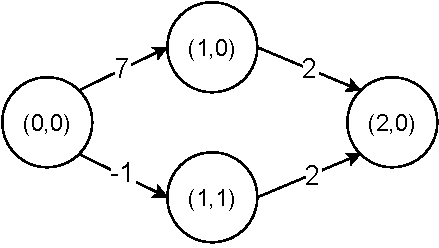
\includegraphics[width=0.4\textwidth]{Basic_Neural_Network.pdf}
%    \caption{A Simple Neural Network}
%    \label{Figure: Simple Neurla}
%
%\end{figure} 
%
%Figure \ref{Figure: Simple Neurla} depicts a feed forward neural network comprising four neurons: $n_0^{0}$, $n_0^{1}$, $n_1^{1}$, and $n_0^{2}$. The weight matrix between layer 0 and layer 1, denoted by $W_{0,1}$, is $[7, -1]^T$, and the bias matrix for layer 1, denoted by $B_{1}$, is $[0, 0]^T$. If we assign a value of 1 to the neuron $n_0^{0}$ (i.e., $v_0^{0}=1$), then the value of the neuron $n_0^{1}$ is $v_0^{1}=7$, as determined by $V_{1} = \phi([7, -1]^{T} \cdot [1] + [0, 0]^{T}) = [7, 0]^{T}$.
%
%
%\subsection{Neural Network Verification }
%In the context of neural network verification, we typically engage with a neural network, posing a ``$\textit{satisfiablility}$'' query to validate or refute a property. The query \(\mathcal{P}\) is structured as a triple, \(\mathcal{P} = \langle \mathcal{N}, \kappa, \lambda \rangle\). Here, \(\mathcal{N}\) denotes the neural network as previously mentioned, while \(\kappa\) and \(\lambda\) represent properties on the input and output neurons, respectively. 
%
%$\kappa$ is defined as a conjunction of linear constraints applied to the input neurons. Correspondingly, $\lambda$ is also expressed as a conjunction of linear constraints targeting the output neurons. Our objective is to verify boolean properties formulated as $\forall x \in X,\textit{ } y < c$. However, for the purpose of assessing the validity of these properties, we transform our $\lambda(y)$—the conjunction of constraints on our output variables—into the negation of $y < c$, represented as $y \geq c$, where $y$ denotes the output of the neural network. To achieve this transformation, we introduce additional neurons into the network, resulting in a modified network structure with a singular output neuron. This transformation of the Neural Network $\mathcal{N}$ proves advantageous for subsequent Inc/Dec classification, which is described in the subsequent section 2.3.1.
%
%Our query is constructed as a boolean formula \(\mathcal{P}(x) \equiv \kappa(x) \land \lambda(\mathcal{N}(x))\). Since we are looking for validity we use the negation of the output property and seek an `UNSAT'. The solver is presented with the formula \(\exists x \in X, \mathcal{P}(x)\), where \(X\) is the domain of the input. If our solver responds with `SAT' to this query, it indicates that we have identified a counterexample, and our property does not hold. Conversely, an `UNSAT' result signifies the validity of our original property.
%
%
%\subsection{Counter-example guided abstraction and refinement}
%To aid and expedite the verification queries, we employ a strategy to simplify our neural network by reducing the number of neurons. Our approach involves constructing an over-approximate network, denoted as $\mathcal{N''}$, where the output value, $\mathcal{N''}(x)$, consistently exceeds the value computed by the original network, $\mathcal{N}(x)$, i.e ($\forall x \in X, \hspace{1mm} \mathcal{N''}(x) \geq \mathcal{N}(x)$), where $X$ is our input domain. This simplification is undertaken because our property which is expressed as $\forall x \in X, \hspace{1mm} \mathcal{N}(x) < c$ can then be proven by determining the unsatisfiability of $\exists x \in X, \hspace{1mm}\mathcal{N''}(x) \geq c$. If the answer to this question is `Yes,' then it implies that $\forall x \in X, \hspace{1mm} \mathcal{N}(x) < c$ holds, as evidenced by ($\forall x \in X, \hspace{1mm} \mathcal{N''}(x) \geq \mathcal{N}(x)$).
%
%
%
%\subsubsection{Increment Decrement Splitting}
%To aid in the process of constructing such an over-approximate network we begin with the creation of an equivalent network, denoted as $\mathcal{N}'$, ensuring that $\mathcal{N'}(x)$ equals $\mathcal{N}(x)$ for all $x$. To build this equivalent network, we perform an `Increment/Decrement' splitting of neurons in our original network $\mathcal{N}$. Upon reflection, it became apparent to us that a two-class classification was more fitting for our needs, deviating from the initially recommended four-class classification outlined in the original work by \cite{b2}.
%Neurons are categorized as `Increment (Inc)' if increasing their values increases the output neuron's value, and as `Decrement (Dec)' if decreasing their values achieves the same result.
%
%\begin{algorithm}[H]
%    \caption{split\_Inc\_Dec}
%    \begin{algorithmic}[1]
%        \State Initialize M, the set of nodes that are marked, to \{out\_node\} and mark out\_node as \textbf{Inc}.
%        \State Let $R$ be the set of nodes with successors in $M$.
%        \State Define $\text{sign(u,v)}$ as the sign of the weight from the node $u$ to $v$.
%        \State Define $\text{Class(v)}$ as $1$ when $v$ is marked as $\textbf{Inc}$, and $-1$ otherwise.
%        \While {\text{node} $\notin M$ and node $\notin$ input\_nodes}
%        \State Pick a node $u$ such that $u \in R-M$
%        \State Suppose $u$ feeds into $x_1,x_2,x_3,..$ and $y_1,y_2,y_3..$ where $\text{sign($u,x_i$)} = \text{Class($x_i$)}$ for all $x_i$, $\text{sign($u,y_i$)} \neq \text{Class($y_i$)}$ for all $y_i$.
%        \State Split $u$ to $u_1$ and $u_2$, where $u_1$ feeds into all the $x_i$ and $u_2$ feeds into all the $y_i$.
%        \State Mark $u_1$ as \textbf{Inc} and $u_2$ as \textbf{Dec}
%        \State Insert $u_1$ and $u_2$ into $M$ and their predecessors into $R$
%        \EndWhile
%        \end{algorithmic}
%\end{algorithm}
%% \begin{algorithm}
%% \caption{splitIncDec}
%% \begin{algorithmic}[1]
%% \Require Graph $G$
%% \State $G.nodes[output\_node]['Inc/Dec']='Inc'$
%
%% \For{$layer$ in $reversed(G.intermediate\_layers)$}
%%     \For{$curr\_node$ in $layer$}        
%%         \For{$node$ in $G.adj[curr\_node]$}
%%             \State inc\_node, dec\_node are Inc/Dec copies of the curr\_node neuron
%%             \State $wgt = G.adj[node]['weight']$
%%             \If{$wgt > 0$ \textbf{and} $G.nodes[node]['inc/dec']=='inc'$}
%%                 \State $G.add\_edge(inc\_node, node, weight = wgt)$
%%             \ElsIf{$wgt < 0$ \textbf{and} $G.nodes[node]['inc/dec']=='dec'$}
%%                 \State $G.add\_edge(inc\_node, node, weight = wgt)$
%%             \ElsIf{$wgt < 0$ \textbf{and} $G.nodes[node]['inc/dec']=='inc'$}
%%                 \State $G.add\_edge(dec\_node, node, weight = wgt)$
%%             \ElsIf{$wgt > 0$ \textbf{and} $G.nodes[node]['inc/dec']=='dec'$}
%%                 \State $G.add\_edge(dec\_node, node, weight = wgt)$
%%             \EndIf
%%         \EndFor
%%     \EndFor
%% \EndFor
%% \end{algorithmic}
%% \end{algorithm}
%
%
%
%\subsubsection{Abstraction}
%
%\begin{figure}[H]
%    \centering
%    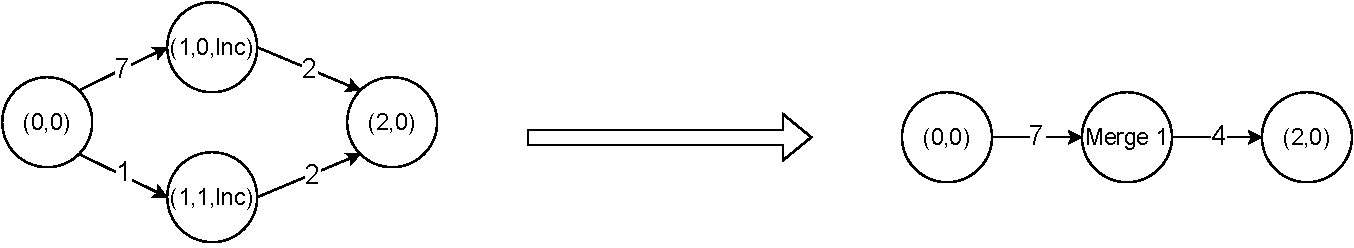
\includegraphics[width=0.9\textwidth]{Abstraction_part1.pdf}
%    \caption{Merging of Increment Neurons}
%    \label{Figure: Merge1}
%    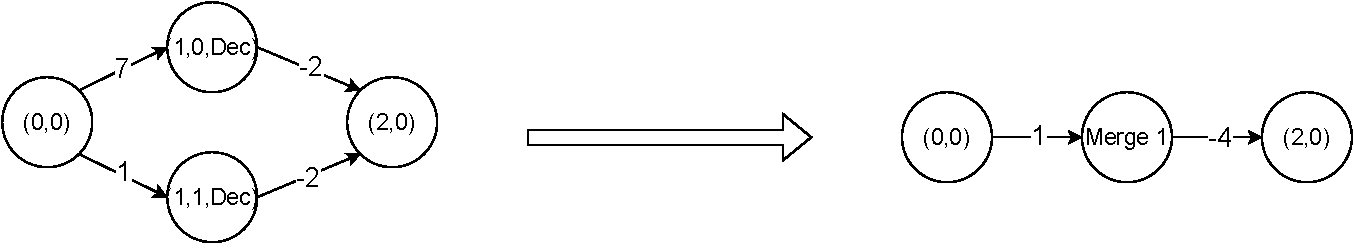
\includegraphics[width=0.9\textwidth]{Abstraction_part2.pdf}
%    \caption{Merging of Decrement Neurons}
%    \label{Figure: Merge2}
%
%\end{figure} 
%The increment/decrement splitting of the neural network $\mathcal{N}$ to the new network $\mathcal{N'}$ changes the structure of the neural network but does not change the value of the output neuron. If we want to construct a neural network $\mathcal{N}''$ which over-approximates the value of the original network $\mathcal{N}$ i.e $\forall x \in X, \hspace{1mm} \mathcal{N''}(x) \geq \mathcal{N}(x)$, then we perform the following steps:
%\begin{enumerate}
%    \item When merging two $\textit{Increment Neurons}$, discard one of those neurons and replace the incoming weight by maximum of all the incoming weights and the outgoing weight by summation of all the outgoing weights. 
%    \item When merging two $\textit{Decrement Neurons}$, discard one of those neurons and replace the incoming weight by minimum of all the incoming weights and the outgoing weight by summation of all the outgoing weights. 
%\end{enumerate}
%
%
%\subsection{Refinement }
%After merging the neurons, we introduce an over-approximation into the new network $\mathcal{N''}$. And since $\mathcal{N''}(x) \geq \mathcal{N}(x)$, there might exist a $x$, for which, $\exists x \in X, \hspace{1mm} \mathcal{N''}(x) \geq c$ but $\nexists x \in X, \hspace{1mm} \mathcal{N}(x) \geq c$. Therefore, if a counter-example `$\beta$' returned is not a valid counter-example, which means, $\mathcal{N''}(\beta) \geq c > \mathcal{N}(\beta)$, then, we must reverse some of the merges performed previously to get a new network which mitigates the extent of the over-approximation for us to get a valid counter-example or to prove that the original property is valid.
%
%In \cite{b2}, the authors employed a Counterexample-Guided Abstraction Refinement (CEGAR) approach to eliminate the spurious counter-examples. They utilized a counter-example ($\beta$) to identify a neuron $n_i^j$ that had been merged into the node `$r$' for refinement. The authors then computed the value $\omega$ which was equal to $|v_i^j(\beta) - r(\beta)| \cdot |w_{n_{i-1,k},n_{i,j}}-w_{n_{i-1,k},r}|$, where $v_i^j(\beta)$ denotes the value of $n_{i,j}$ at the counter-example $\beta$, $r(\beta)$ denotes the value of the representative neuron $r$ at the counter-example $\beta$, $w_{n_{i-1,k},n_{i,j}}$ denotes the weight between a neuron $n_{i-1,k}$ and a neuron $n_{i,j}$. If this value $\omega$ was over a recommended amount $\epsilon$, they proceeded to separate $n_i^j$ from $r$ to potentially eliminate the spurious counter-example $\beta$.
%
%
% In the next section, we present a new method for merging neurons in order to reduce the number of refinement steps, thereby expediting the verification process.
%
%\section{Methodology}
%
%Our methodology involves two broad steps:
%\begin{enumerate}
%    \item Finding a tree structure that represents the order in which neurons should be merged.
%    \item Using that structure to guide a CEGAR approach in order to help reduce number of refinement steps.
%\end{enumerate} 
%
%\subsection{Tree and Merges:}
%
%To establish the merging order of neurons, we create a tree structure wherein leaf nodes represent the original neurons, and non-leaf nodes represent merge groups. The construction of the tree follows a bottom-up approach, prioritizing the merging of similar neurons and delaying the merging of dissimilar ones. Similarity is ascertained through observation vectors. Consider simulating the network with distinct input values and observing the fluctuating values of a particular neuron corresponding to those inputs. The collection of these observed values constitutes an observation vector. 
%
%\begin{figure}[H]
%    \centering
%    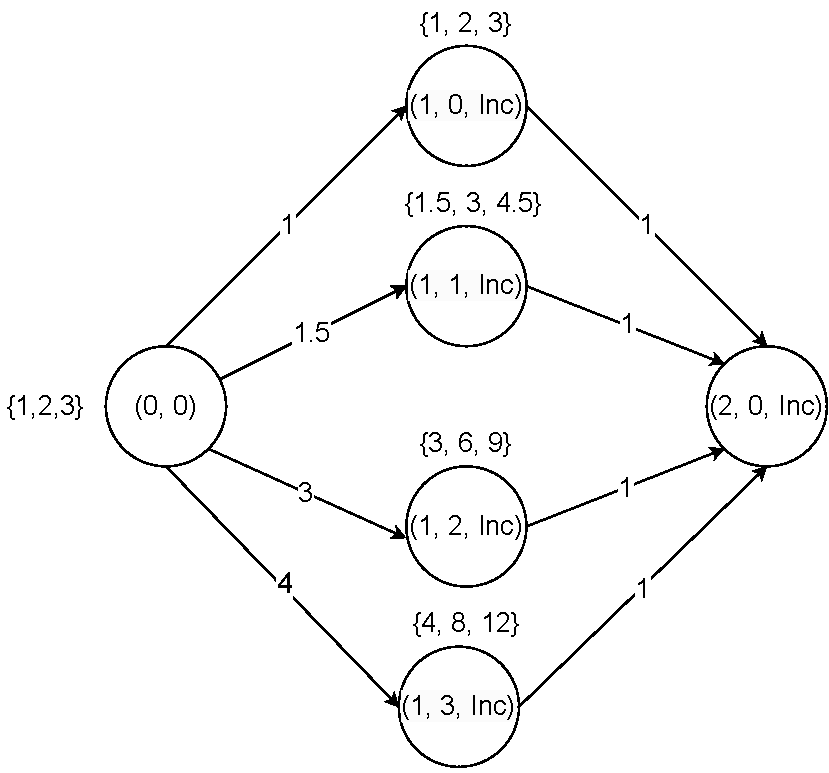
\includegraphics[width=0.5\textwidth]{tree_merges.pdf}
%    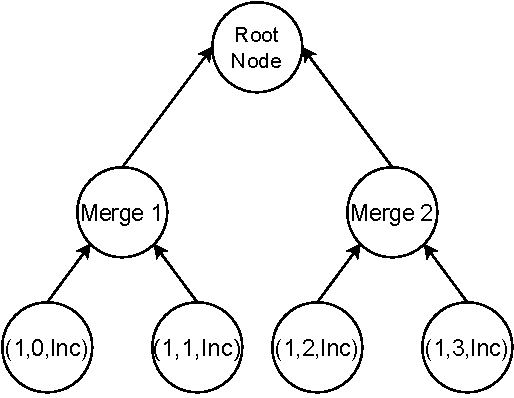
\includegraphics[ width=0.47\textwidth]{Order_of_Merge.pdf}
%    \caption{Order Of Merging}
%    \label{Figure: Order Of Merging}
%\end{figure}
%
%
%In Figure \ref{Figure: Order Of Merging}, when we input values \{1, 2, 3\} to the neuron $n_0^{0}$ at different time instances, we obtain corresponding values \{1.5, 3, 4.5\}, forming the observation vector at neuron $(n_1^{1},Inc)$. For instance, considering three neurons $n_i^{w}$, $n_j^{w}$, and $n_k^{w}$ with observation vectors $\mathcal{\nu}(n_i^{w})$, $\mathcal{\nu}(n_j^{w})$, and $\mathcal{\nu}(n_k^{w})$, the merging sequence adheres to the following conditions: 
%
%If $||\mathcal{\nu}(n_i^{w}) - \nu(n_j^{w})||_{2} \leq ||\nu(n_i^{w}) - \nu(n_k^{w})||_{2}$ and $||\nu(n_i^{w}) - \nu(n_j^{w})||_2 \leq ||\nu(n_j^{w}) - \nu(n_k^{w})||_{2}$, then $n_i^{w}$ and $n_j^{w}$ are initially merged into a representative neuron $\alpha$, followed by the merging of $\alpha$ and $n_k$. Here $||\nu(n_i^{w}) - \nu(n_j^{w})||_{2}$ computes the ``$\textit{Euclidean  Distance}$" between the observation vectors $\nu(n_i^{w})$ and  $\nu(n_j^{w})$.
%
%
%In Figure \ref{Figure: Order Of Merging}, for the first layer, the initial merge would involve the neuron $(n_0^{1},Inc)$ with $(n_1^{1},Inc)$, forming $\textit{Merge 1}$, then we would combine $(n_2^{1},Inc)$ and $(n_3^{1},Inc)$, forming $\textit{Merge 2}$. Finally we combine $\textit{Merge 1}$ and $\textit{Merge 2}$ into the root node. 
%
%As we progress up the tree, the degree of over-approximation rises. This is due to the increasing difference between observation vectors as we ascend. Therefore, the sub-trees closer to the root are indicative of coarser merges, whereas the ones farther from the root represent finer merges. 
%
%
%
%\subsection{Using Counter-Examples to make cuts in the Tree} 
%We are guided by this tree as a prospective refinement method. Starting with the entire tree where everything is merged. When the solver detects a spurious counterexample `$\beta$', we leverage it to refine the network. This process commences by identifying the ``culprit neuron $\gamma$'' selected for refinement. A ``culprit neuron'' in a merge group is selected on the basis of how much the neuron contributed to the output. If change in output of  neuron changes the value of the output neuron significantly then that neuron is a good candidate for ``culprit neuron". 
%
%Following this, we reverse all merges dependent on the culprit neuron $\gamma$. Therefore, refinement essentially involves finding a cut-point in the tree, precisely where all merges dependent on the culprit neuron $\gamma$ are undone. Each cut produces a set of trees, the merge groups then consist of neurons in the leaf nodes of the  these trees. Therefore finding new merge groups for refinement is therefore just finding a cuts in the tree.
%
%\begin{figure}
%    \centering
%    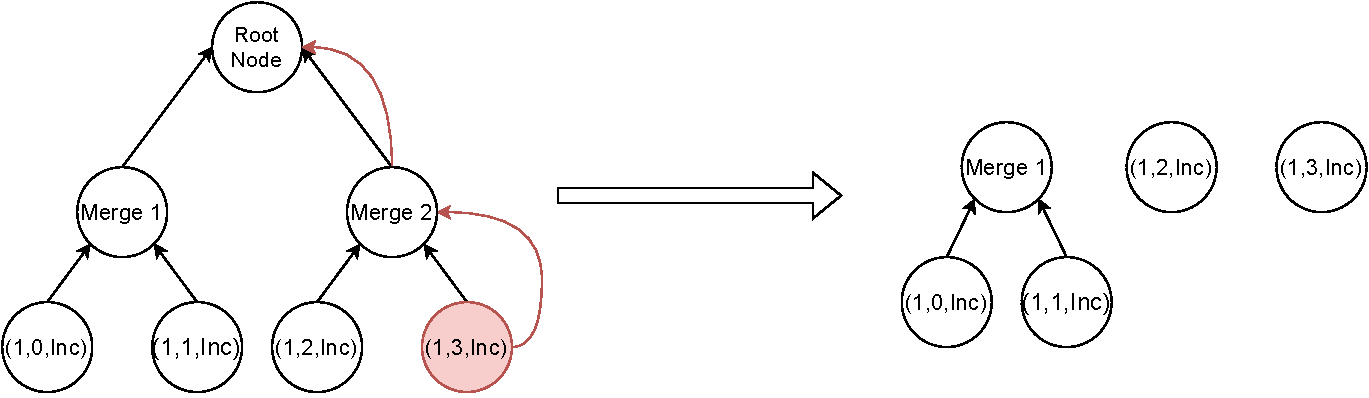
\includegraphics[width = 0.9\textwidth]{_before and after cut.pdf }
%    \caption{Trees and Cuts}
%    \label{Figure 2}
%\end{figure}
%
%Consider Figure \ref{Figure 2}, illustrating the merging sequence of neurons $(n_0^{1}, Inc)$, $(n_1^{1}, Inc)$, $(n_2^{1}, Inc)$, and $(n_3^{1}, Inc)$. If, for instance, the neuron $(n_3^{1}, Inc)$ is identified as the problematic neuron based on a counter-example, we will reverse all the merges dependent on the $(n_3^{1}, Inc)$ neuron, including $\textit{Merge 2}$ and the $\textit{Root Node}$ merge. Consequently, after implementing this reversal indicated in Figure \ref{Figure 2}, our refinement phase will yield three distinct merge groups. The first merge group comprises two neurons, namely $(n_0^1, Inc)$ and $(n_1^1, Inc)$. The second merge group and the third merge have single neurons $(n_2^1, Inc)$ and $(n_3^1, Inc)$, respectively.
%
%\subsection{Culprit Neurons} 
%
%A neuron, denoted as $\gamma$, is designated as a culprit neuron within a specific layer when absolute value of the product of the difference between $(v_{Rep(\gamma)}$ and $v_{\gamma})$ and the effective weight is maximized.
%
%
%$||(v_{Rep(\gamma)} - v_{\gamma})||_{2} \cdot |(\textit{effective\_weight})|$
%
%In this context, $Rep$ signifies the representative neuron for neuron $\gamma$, $v_{\gamma}$ represents the value of the neuron $\gamma$ at counter-example $\beta$ and $\textit{effective\_weight}$ represents the how much does the value of output neuron changes with respect to change in the value of the neuron under consideration, essentially corresponding to the ``$\textit{gradient}$'' at that particular counter-example ``$\beta$''.
%
%\begin{algorithm}
%    \caption{Finding Cuts in the Tree (find\_new\_merge\_groups)}
%    \begin{algorithmic}[1]
%        \State $\gamma= \arg \max_i \|v_{Rep(i)} -v_i \|_2 \cdot | \textit{effective\_weight}| $ 
%        \State Find a sequence of nodes, $t_1,t_2,t_3,..,t_k$ representing a  path from $t_1=$root to $t_k=\gamma$.
%        \State Remove the nodes $t_1,t_2,..,t_{k-1}$ denoting the merges dependent on $\gamma$ through this path, leading to our connected tree being split into a collection of disconnected sub-trees.
%        \State New merge groups are the leaf nodes in our disconnected graph.
%    \end{algorithmic}
%    \hspace*{\algorithmicindent} \textbf{Output} New Merge Groups
%\end{algorithm}
%
%\subsection{Optimality of the Trees}
%Our objective is to determine the most efficient order for merging neurons, minimizing the introduction of over-approximation at each step. This approach aims to avoid creating networks with excessive over-approximation, which could lead to the generation of spurious counter-examples in response to queries. Opting not to mitigate over-approximation at each step would result in an increased number of refinement steps. This essentially entails making additional solver calls, incurring significant costs to eliminate the spurious counter-examples.
%
%
%Nevertheless, during the initial merging process (until saturation is reached), the root node ``$\rho$'' will exhibit the same level of over-approximation across all conceivable merging scenarios—for all possible tree sequences. Nevertheless, when we descend one level down the tree to explore the children nodes of our original root node $\rho$ for the purpose of identifying a cut for refinement, we discover varying levels of over-approximation manifesting in the root nodes of the resultant sub-trees. These differences are a result of the different merging scenarios pursued to construct those individual trees.
%
%\begin{algorithm}[H]
%\caption{Cluster Merging Algorithm (find\_abstraction\_tree)}
%\label{Cluster Merging Algorithm}
%\begin{algorithmic}[1]
%    \State Initialize every simulated distance vector as a singleton cluster.
%    \State Initialize $C=\{v_1,v_2,v_3,..\}$ as the set of singleton clusters.
%    \State Initialize a Binary Tree $T$ with leaves as $\{(n_1),(n_2),(n_3),..\}$ corresponding to $\{v_1,v_2,v_3,..\}$.
%    \State Initialize $V$ as a set of visited nodes, empty at first.
%    
%    \Function{MergeFunction}{$u, v$}
%        \If{All nodes are classified as \textbf{Inc}}
%        {
%        
%            \Return $\max(u, v)$
%        }
%        \Else{ }
%        {
%        
%            \Return $\min(u, v)$
%        }
%        \EndIf
%    \EndFunction
%    
%    \While{$|C|>1$}
%        \State $v_j, v_j = \arg\min_{\substack{a, b \in C}} \| a - b \|_2$
%        \State Set $w=\text{MergeFunction}(v_i,v_j)$
%        \State Let nodes from $T$ not in $V$ corresponding to $v_i,v_j$ be $m_i$ and $m_j$
%        \State Remove $v_i,v_j$ from $C$ and add $w$ to $C$.
%        \State Make $(m_i \cup m_j)$ the parent of $(m_i)$ and $(m_j)$ in tree $T$
%        \State Add $m_i$ and $m_j$ to $V$.
%    \EndWhile
%\end{algorithmic}
%\end{algorithm}
%
%While the optimal tree, representing the optimal merging sequence, can aid in the refinement process by guiding the reversal of merges, finding such an optimal tree poses is extremely challenging. Even when dealing with only `n' Increment (Inc) neurons that have been merged to saturation, the total number of possible trees is given by $(2n-3)!!$, making the task of determining the truly optimal tree from these options extremely challenging.
%
%Since finding this ideal tree is a challenging task, we employ hierarchical clustering (Algorithm \ref{Cluster Merging Algorithm}) as an approach to approximate and derive such a tree. Initially, we simulate our network using a set of `$k$' inputs. Subsequently, we employ cluster analysis on these `$k$' points to construct a hierarchical arrangement of clusters. This process initiates with data points corresponding to simulated values (observation values in the observation vector) of a neuron  forming their own cluster. The clusters are then systematically combined based on their similarity, thereby generating a hierarchy of clusters. The choice of similarity measure is the ``$distance \hspace{1mm} metric$" between clusters. We have used ``$Euclidean \hspace{1mm} Distance$" as our distance metric. Given that the data points to perform this hierarchical clustering originate from the values of the simulated neurons, this hierarchical clustering effectively reflects the methodology we employ to merge the neurons.
%
%For example, in Figure \ref{Figure: Order Of Merging}, we conducted a simulation of our network on three data points. Subsequently, we examined the observation vectors corresponding to these points. Utilizing the hierarchical clustering algorithm, the initial selection for merging  will involve $(n_0^{1}, Inc)$ and $(n_1^{1}, Inc)$ because of the fact that their Euclidean distance is minimum. This forms $\textit{Merge 1}$ in Figure \ref{Figure: Order Of Merging}. The observation vector for $\textit{Merge 1}$ ($\nu_\textit{Merge1 }$) is the max of the $\nu((n_0^{1}, Inc))$ and $\nu((n_1^{1},Inc))$ which is \{1.5, 3, 4.5\}. For decrement nodes the observation vector would be minimum of the observation vector of the corresponding decrement nodes. The next merging step involved selecting $\nu((n_2^{1}, Inc))$ and $\nu((n_3^{1}, Inc))$ and merging these two neurons, representing $\textit{Merge 2}$ in Figure \ref{Figure: Order Of Merging}. The observation vector for $\textit{Merge 2}$ is now \{4, 8, 12\}. Ultimately, the Merge1 merge group is merged with the $\textit{Merge 2}$ merge group to create the Root Node in our network.
%
%\begin{figure}[H]
%    \centering
%    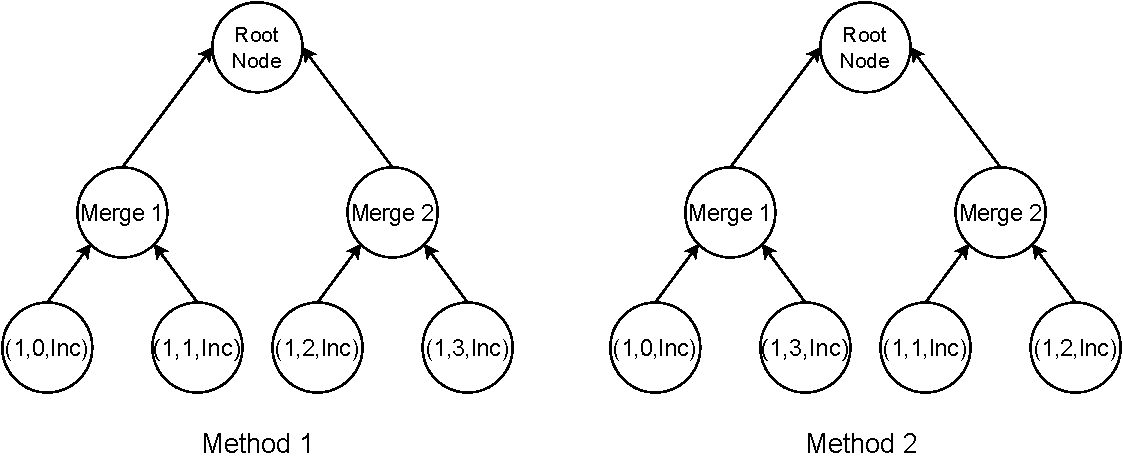
\includegraphics[width = 0.9\textwidth]{good_vs_bad_merges.pdf}
%    \caption{Ways of Merging}
%    \label{Figure 3}
%\end{figure}
%
%This approach of merging neurons based on similarity proves advantageous as it helps in reducing number of refinement steps. For instance, consider the task of checking whether $\forall v_{0}^{0} \in [0, 1]$ implies $v_{0}^{2} < 10$. If we had the neuron $(n_{3}^{1}, Inc)$ as the culprit neuron and then if we follow the second merging approach depicted in Figure \ref{Figure 3}, then we would have been compelled to reverse both $\textit{Merge 1}$ and $\textit{Merge 2}$. However, by employing the first merging approach, undoing only the $\textit{Merge 2}$ becomes sufficient, resulting in a reduction in the number of refinement steps required.
%
%
%\subsection{Overall Algorithm}
%\begin{algorithm}[H]
%    \caption{Overall Algorithm}
%    \label{Overall Algorithm}
%    \begin{algorithmic}[1]
%        \State $\mathcal{N'}$ = split\_Inc\_Dec($\mathcal{N}$)
%        \State $\mathcal{N''}$ = abstract\_network($\mathcal{N'}$)
%        \State simulation\_dict = simulate\_network($\mathcal{N'}$)
%        \State $\mathcal{T}$ = find\_abstraction\_tree($\mathcal{N'}$, $simulation\_dict$)
%        \If{verify($\mathcal{N''}$, $\kappa$, $\lambda$) is UNSAT}{
%
%            \Return Property Holds
%            }
%        \Else
%            \State Extract counter-example $\beta$
%            \If{$\beta$ is not a spurious counter-example}
%            {
%
%                \Return ($\beta$, Property Violated)
%            }
%            \Else
%                \State Find culprit neuron $\gamma$
%                \State $merge\_groups$ = find\_new\_merge\_groups($\mathcal{T, \gamma}$)
%                \State $\mathcal{N''} = get\_abstract\_network(merge\_groups)$
%                \State \textbf{goto} step 5
%            \EndIf
%        \EndIf
%    \end{algorithmic}
%\end{algorithm}

%\end{flushleft}

\printbibliography
    
\end{document}
 

